\chapter{Knot selection in spline models: cocaine dependence}
\label{applications-splines_knot_loc}

For many conditions prevalence varies substantially as a function of
age.  Other epidemiological parameters, such as incidence and
excess-mortality hazards, often have important age patterns as well.
The spline models introduced in Chapter~\ref{theory-age_pattern_model}
provide a flexible framework for representing this age-dependent
phenomena.  However, there are some important modeling decisions
necessary in this process.  The following examples from estimating the
age-specific prevalence of cocaine dependence illustrate the
importance of choosing knot locations and choosing smoothing levels
appropriately in a setting where the data speak relatively precisely
about the level and age pattern of the condition.

The American Psychiatric Association's Diagnostic and Statistical Manual version IV
(DSM-IV) recognizes cocaine dependence as fulfilling three or more of the
following seven dependence criteria during any time in the
same twelve-month period: \cite{american_psychiatric_association_diagnostic_2000, wagner_first_2002}
    \begin{itemize} \label{page:app-substance_dependence}
        \item tolerance to effects of cocaine (typically assessed through either the same amount of cocaine having less effect or requiring greater amounts to obtain the desired effect);
        \item withdrawal symptoms after use ceases;
        \item usage over longer period or in larger quantities than intended;
        \item persistent desire or unsuccessful efforts to control
          cocaine use;
        \item spends a lot of time to obtain, use, or recover
          from effects of cocaine;
        \item reduction of important social, occupational, or recreational
          activities because of cocaine use;
        \item continues cocaine use despite knowledge of
          physiological or psychological problems induced by cocaine
          use.
    \end{itemize}

Despite a large body of data on cocaine \emph{use}, there are comparatively few
data available on the descriptive epidemiology of cocaine
\emph{dependence}.\cite{degenhardt_what_2011} Systematic review for cocaine
dependence identified $28$ prevalence data points,
covering $3$ GBD 2010 Study regions.  For this example, we have restricted our attention
to only data from the United States of America (Figure~\ref{fig:app-cocaine_data}).

    \begin{figure}[h]
        \begin{center}
            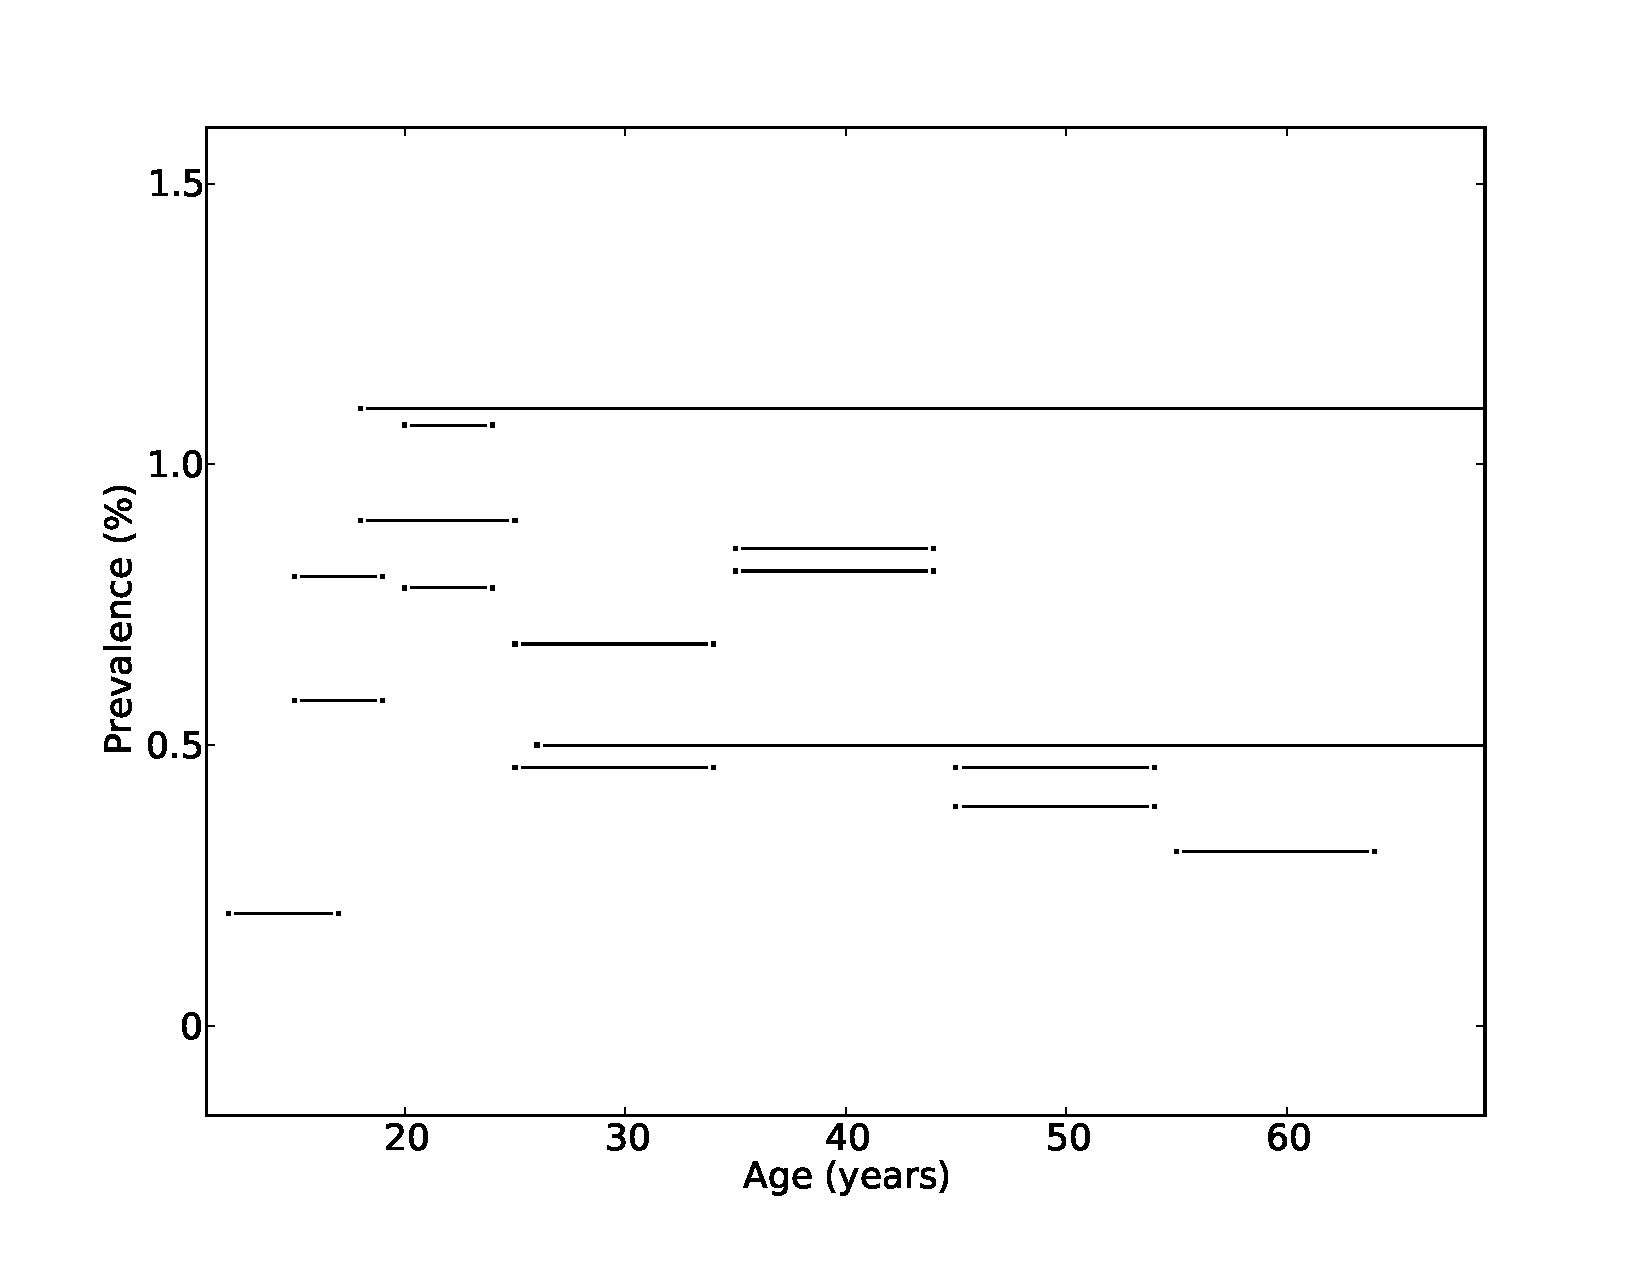
\includegraphics[width=\textwidth]{cocaine_dependence-data.pdf}
            \caption{Prevalence data for cocaine dependence in the
              United States of America. Each horizontal bar represents
              a single data point extracted in systematic review.  The
              left and right endpoints indicate the start and end ages
              of the age interval for a data point, while the level of
              prevalence is represented by the distance of the bar
              above the $y$-axis.}
            \label{fig:app-cocaine_data}
        \end{center}
    \end{figure}

As discussed in Chapter~\ref{theory-age_pattern_model}, we model
age-specific hazards with spline models.  To be more specific, in this
case, the spline model takes the form of a continuous, piecewise
linear function, with selected ``knots'' where the function is non-linear.
These knots partition the age range
into intervals, and the choice of knots can be influential on the
resulting estimates.  In a setting where data is \emph{not} sparse and
noisy, estimates will not be very sensitive to choice of knots.
However, when working with sparse and noisy data, the number and
location of knots are important decisions as they can influence the
model results substantially.  Thus, the number of knots and locations
should be chosen a priori using expert knowledge concerning the
disease being modeled.  It is also
important to consider additional knots and alternative configurations
of knots as a sensitivity analysis.

To demonstrate the importance of the number of knots in a spline
model, we compare three models with differing numbers of knots in
Figure~\ref{fig:app-cocaine_knots}.  The 7 knot model for cocaine
dependence has knot set $\{15, 20, 25, 30, 40, 50, 65\}$, based on the theory that prevalence is zero in childhood,
changes rapidly during early adulthood, and then changes less rapidly
in older ages.  The age pattern of prevalence estimated with this
model is shown as a solid line.

Another model we consider is a 4 knot model, using the knot set $\{15, 25,
40, 65\}$.  The estimates from this model, shown as a dotted line,
show how, seemingly paradoxically, fewer knots can lead to more
extreme estimates for certain ages.

We also fit a model with 11 knots, using knots spaced every five years from
ages 15 to 65.
The estimates from this model are shown as a dashed line in
Figure~\ref{fig:app-cocaine_knots}.  When data is sparse, adding
additional knots allows for estimates that follow the vagaries of the
data more closely, which may not be desired.  Smoothing priors for the
penalized spline model can address this, which will be examined next.

    \begin{figure}[h]
        \begin{center}
            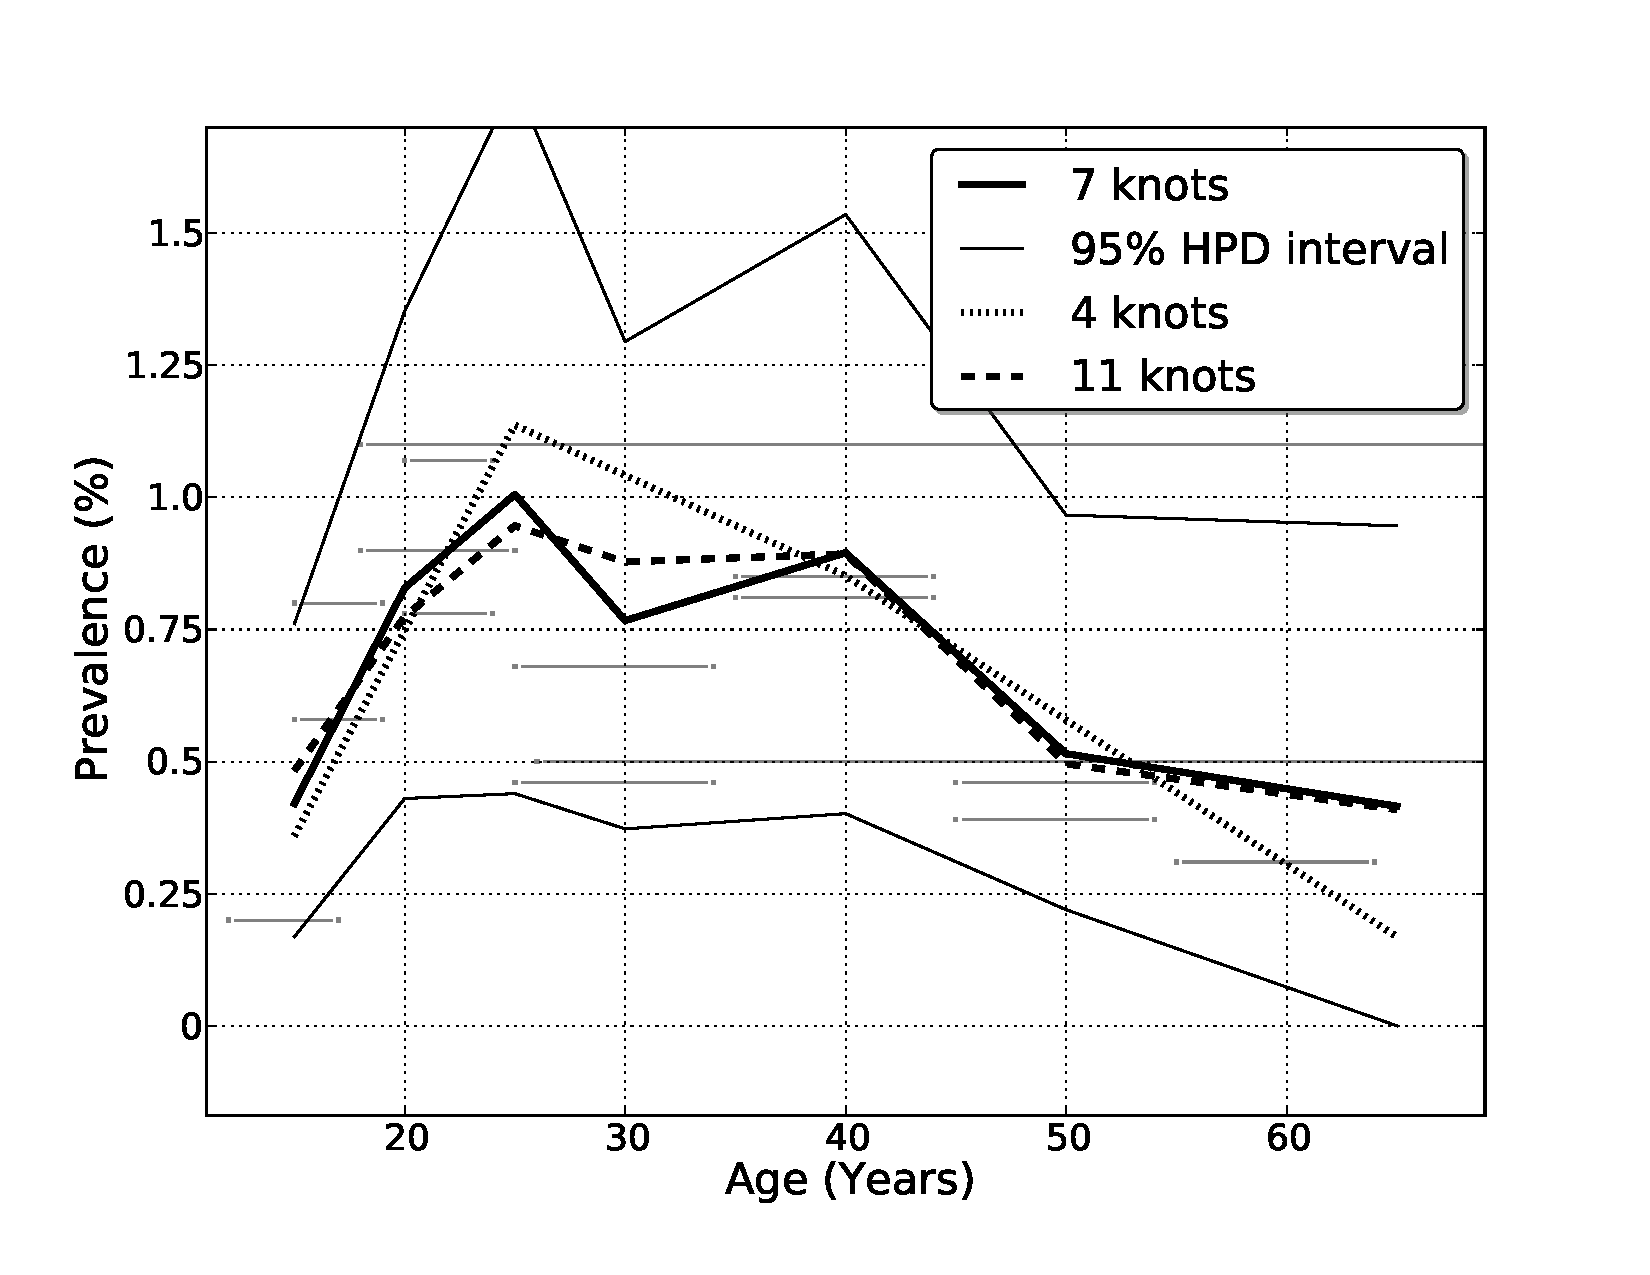
\includegraphics[width=\textwidth]{applications/cocaine_dependence-knots.pdf}
            \caption{Prevalence estimates of cocaine dependence in the United
              States of America using a spline model with 4, 7 and 11 knots. }
        \label{fig:app-cocaine_knots}
        \end{center}
    \end{figure}

The penalized spline model introduces an additional term to the model
prior to encode the belief that the age pattern is not too wiggly.
With the judicious choice of the smoothness hyperparameter, the model
can include more knots without using them to chase the noise around in
the noisy data.  The effects of four values of the smoothing parameter
are shown in Figure~\ref{fig:app-cocaine_smoothing}.  The smaller the
parameter, the smoother the estimated age pattern, hence, the less
influential the position of the knots.  However, too much smoothing
leads to overcompression of the prevalence estimates with estimates
that are not representative of the data.

    \begin{figure}[h]
        \begin{center}
            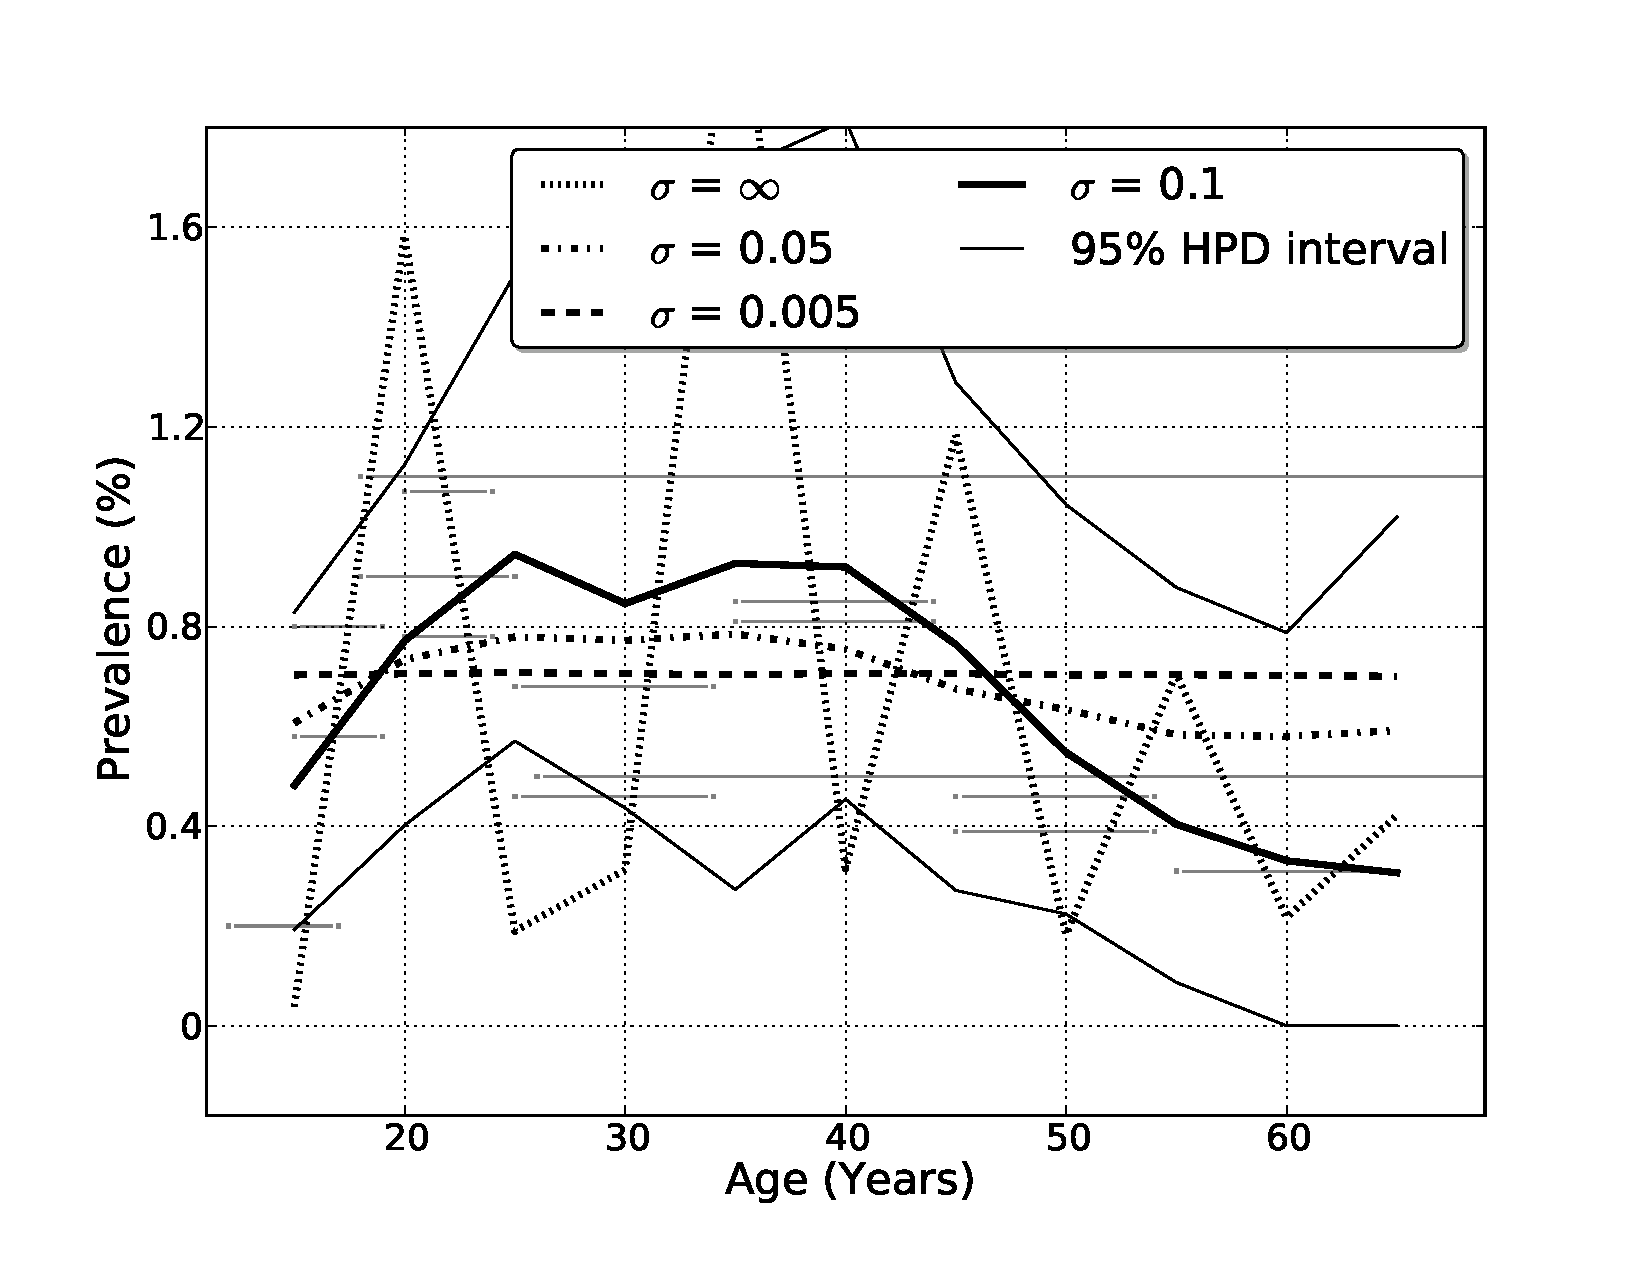
\includegraphics[width=\textwidth]{applications/cocaine_dependence-smoothing.pdf}
            \caption{Prevalence estimates from the model with knots every five years
              using a penalized spline model with a smoothing
              parameter $\sigma$. }
        \label{fig:app-cocaine_smoothing}
        \end{center}
    \end{figure}

As shown by the figures above, knot location and smoothing
hyperparameter selection can be an influential part of the model.
From the sensitivity analysis in Figure~\ref{fig:app-cocaine_knots},
it appears that there is nothing to gain from adding additional
knots to the model, although it is possible to do so if an appropriate
smoothing parameter is included also.  In the next chapter, we will
consider a case where the data does not have such a clear story to
tell about the age pattern.
